
% This LaTeX was auto-generated from MATLAB code.
% To make changes, update the MATLAB code and republish this document.

\documentclass{article}
\usepackage{graphicx}
\usepackage{color}

\sloppy
\definecolor{lightgray}{gray}{0.5}
\setlength{\parindent}{0pt}

\begin{document}

    
    
\section*{Filter 50/60 Hz signal from ECG simulated data}

\begin{par}
This script demonstrate how to filter a noisy ECG signal. Over the simulated ECG signal is added baseband noise, white noise and power line hum.
\end{par} \vspace{1em}

\subsection*{Contents}

\begin{itemize}
\setlength{\itemsep}{-1ex}
   \item User controlled variables
   \item Create ECG simulated signal
   \item Low pass filtering and high pass filtering
   \item LMS 2 tap
   \item LMS 4 taps
   \item LMS n taps
   \item Output plots
\end{itemize}


\subsection*{User controlled variables}

\begin{verbatim}
LPF_cutoff = 25; %ECG signal band => between 10 Hz and 25 Hz
HPF_cutoff = 1; % Baseline wander frequency is lower than 1Hz. Can be higher in special conditions (running)
LMS_conv = 0.009;

% noise amplitudes
Noise_amplitude = 0.020;
Mains_interference_amplitude = 8;
Baseline_wander_amplitude = 1;

f_baseline = 0.2;
f_interference = 50.5; % power line frequency

Fs = 50 * 16;  %sample rate
dt=1/Fs;
t=0:dt:16;

ref = sin(2*pi*f_interference*t);

% Insert a frequency offset for the interference signal
f_offset1 = 0;
f_offset2 = 0;
interference_noise = Mains_interference_amplitude * sin (2*pi*(f_interference-f_offset1)*t) + ...
                     Mains_interference_amplitude * 0.2 *sin(2*pi*(f_interference-f_offset2)*t);
\end{verbatim}


\subsection*{Create ECG simulated signal}

\begin{verbatim}
Hearth_rate = 75;
ECG_period = Hearth_rate/60;
QRS_complex_duration = 0.08; % QRS complex duration is between 0.08 - 0.12 seconds
PR_duration = 0.12;  % PR duration is between 0.12 -0.20 seconds
QT_duration = 0.40; % QT duration is between 0.35 - 0.43 seconds
\end{verbatim}
\begin{par}
\textbf{Create QRS complex shape}
\end{par} \vspace{1em}
\begin{verbatim}
QRS_t = 0:dt:QRS_complex_duration;
QRS_f = 1/QRS_complex_duration;
QRS_waveform = sin(2*pi*QRS_f/2*QRS_t).*(QRS_t<=QRS_complex_duration);
\end{verbatim}
\begin{par}
\textbf{Create PR interval shape}
\end{par} \vspace{1em}
\begin{verbatim}
PR_t = 0:dt:PR_duration;
PR_f = 1/PR_duration;
PR_waveform = 0.2*sin(2*pi*PR_f/2*PR_t).*(PR_t<=PR_duration);
\end{verbatim}
\begin{par}
\textbf{Create QT interval shape}
\end{par} \vspace{1em}
\begin{verbatim}
QT_t = 0:dt:QT_duration;
QT_f = 1/QT_duration;
QT_waveform = 0.2*sin(2*pi*QT_f/2*QT_t).*(QT_t<=QT_duration);
\end{verbatim}
\begin{par}
\textbf{Create a vector that holds the exact location of the ECG pulse.}
\end{par} \vspace{1em}
\begin{verbatim}
time_location = double(0==mod(t,ECG_period));
\end{verbatim}
\begin{par}
\textbf{Create PR interval with respect to QRS complex position}
\end{par} \vspace{1em}
\begin{verbatim}
ECG_PR = conv(circshift(time_location,[0, -ceil(PR_duration/dt + PR_duration/(2*dt))]), PR_waveform);
ECG_PR = ECG_PR(1:length(ECG_PR) - length(PR_waveform) + 1);
\end{verbatim}
\begin{par}
\textbf{Create QT interval with respect to QRS complex position}
\end{par} \vspace{1em}
\begin{verbatim}
ECG_QT = conv(circshift(time_location,QT_duration/(2*dt)), QT_waveform);
ECG_QT = ECG_QT(1:length(ECG_QT) - length(QT_waveform) + 1);
\end{verbatim}
\begin{par}
\textbf{Repeat QRS complex according to ECG\_period.}
\end{par} \vspace{1em}
\begin{verbatim}
ECG_waveform = conv(time_location, QRS_waveform);
\end{verbatim}
\begin{par}
\textbf{Merge signals PR\_QRS\_QT}
\end{par} \vspace{1em}
\begin{verbatim}
ECG_waveform = ECG_waveform(1:length(ECG_waveform) - length(QRS_waveform) + 1) + ECG_PR + ECG_QT;
\end{verbatim}
\begin{par}
\textbf{Add signal noise: random noise, interference noise and baseline noise}
\end{par} \vspace{1em}
\begin{verbatim}
ECG_waveform_noise = ECG_waveform + Noise_amplitude * randn(size(t));
ECG_waveform_interference = ECG_waveform_noise + interference_noise;
ECG_waveform_final = ECG_waveform_interference + Baseline_wander_amplitude * sin(2*pi*f_baseline*t);
\end{verbatim}


\subsection*{Low pass filtering and high pass filtering}

\begin{verbatim}
[b,a] = butter(2, LPF_cutoff/(Fs/2));
%freqz(b,a)
ECG_LPF = filter(b, a, ECG_waveform_final );

[b,a] = butter(2, HPF_cutoff/(Fs/2),'high');
%freqz(b,a)
ECG_HPF = filter(b, a, ECG_LPF );
\end{verbatim}


\subsection*{LMS 2 tap}

\begin{par}
Fs = 60*16 = 960 hz = 1.04 ms 16.66 ms/2 = 8.33 ms =\ensuremath{>} 4 samples for 90 degree phase shift
\end{par} \vspace{1em}
\begin{verbatim}
% Fs=50*16 = 800 hz = 1.25 ms
% 50 hz -> 20ms => 20/1.25 = 16 samples/cycle => 16/4 = 4 -> 4 samples
% represents 90 degree phase shift

% narrow band filter that works only with frequencies near f_interference
% 2 tap filter - adjust b1 and b2 coefficients for in phase ref(i) and 90 degree
% phase shift ref(i-4) signal

% if interference signal from ECG_HPF would be in phase with the ref signal
% then b2 would be 0 and b1 would be Mains_interference_amplitude/ref_amplitude.

b1 = 0;
b2 = 0;

for i=5:length(t)

    ECG_out(i) = ECG_HPF(i) - (b1*ref(i) + b2*ref(i-4)) ;
    %b1 = b1 + LMS_conv*ECG_out(i)*sign(ref(i));
    %b2 = b2 + LMS_conv*ECG_out(i)*sign(ref(i-4));
    b1 = b1 + LMS_conv*ECG_out(i)*ref(i);
    b2 = b2 + LMS_conv*ECG_out(i)*ref(i-4);

end
\end{verbatim}


\subsection*{LMS 4 taps}

\begin{verbatim}
a1 = 0;
a2 = 0;
a3 = 0;
a4 = 0;
for i=13:length(t)

    ECG_4tap(i) = ECG_HPF(i) -  (a1*ref(i) + a2*ref(i-4) + a3*ref(i-8) + a4*ref(i-12));
    a1 = a1 + LMS_conv*ECG_4tap(i)*(ref(i));
    a2 = a2 + LMS_conv*ECG_4tap(i)*(ref(i-4));
    a3 = a3 + LMS_conv*ECG_4tap(i)*(ref(i-8));
    a4 = a4 + LMS_conv*ECG_4tap(i)*(ref(i-12));

end
\end{verbatim}


\subsection*{LMS n taps}

\begin{verbatim}
n = 20;
h = zeros(1,n+1);
offset = 0:-1:-n;
for i=n+1:length(t)
    % keep a history buffer
    buffer = ref(i+offset);
    ECG_ntap(i) = ECG_HPF(i) - dot(h,buffer);
    h = h + LMS_conv * ECG_ntap(i) * buffer;
end

% smoothdata - not mandatory, just for eye comparation
% ECG_out  = smoothdata(ECG_out);
% ECG_4tap = smoothdata(ECG_4tap);
% ECG_ntap = smoothdata(ECG_ntap);
\end{verbatim}


\subsection*{Output plots}

\begin{par}
\textbf{ECG signal filtering when interference frequency is equal to reference signal 50/60Hz}
\end{par} \vspace{1em}
\begin{verbatim}
figure
subplot(4,1,1);
plot(t,ECG_waveform_final);
title("ECG signal with random noise, power line noise and baseline noise");
subplot(4,1,2);
plot(t,ECG_LPF);
title("ECG signal after low pass filtering");
subplot(4,1,3)
plot(t,ECG_HPF);
title("ECG signal after high pass filtering");
subplot(4,1,4);
plot(t,ECG_out,'y');
title("ECG signal after LMS filtering");
hold on
plot(t,ECG_waveform,'r');
hold on
plot(t,ECG_4tap,'b');
hold on
plot(t,ECG_ntap,'black');
legend('Filtered signal 2LMS','Simulated signal', 'Filtered signal 4LMS', 'Filtered signal NLMS');
set(gcf,'Position',[380 80 800 680]);
saveas(gcf,'ECG_filtering.png');
\end{verbatim}

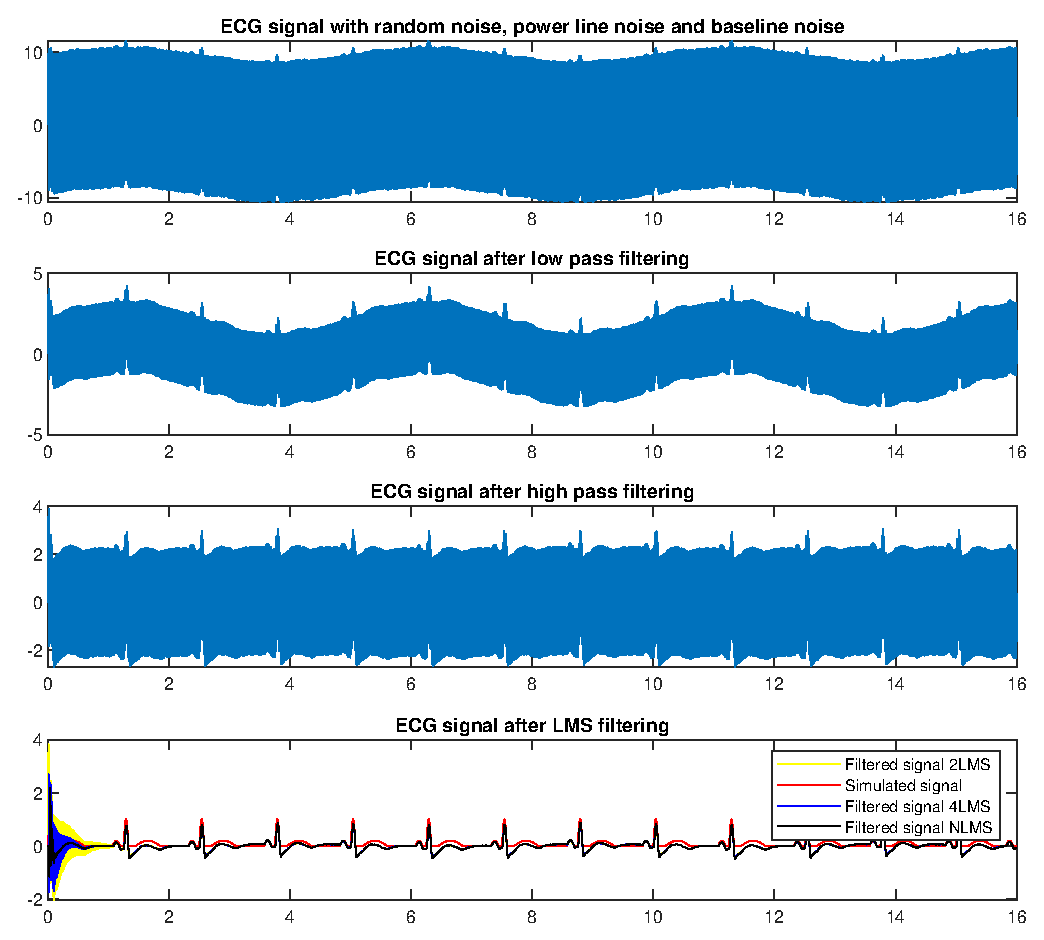
\includegraphics [width=4in]{Filter_power_line_ECG_Vlad_01.eps}
\begin{par}

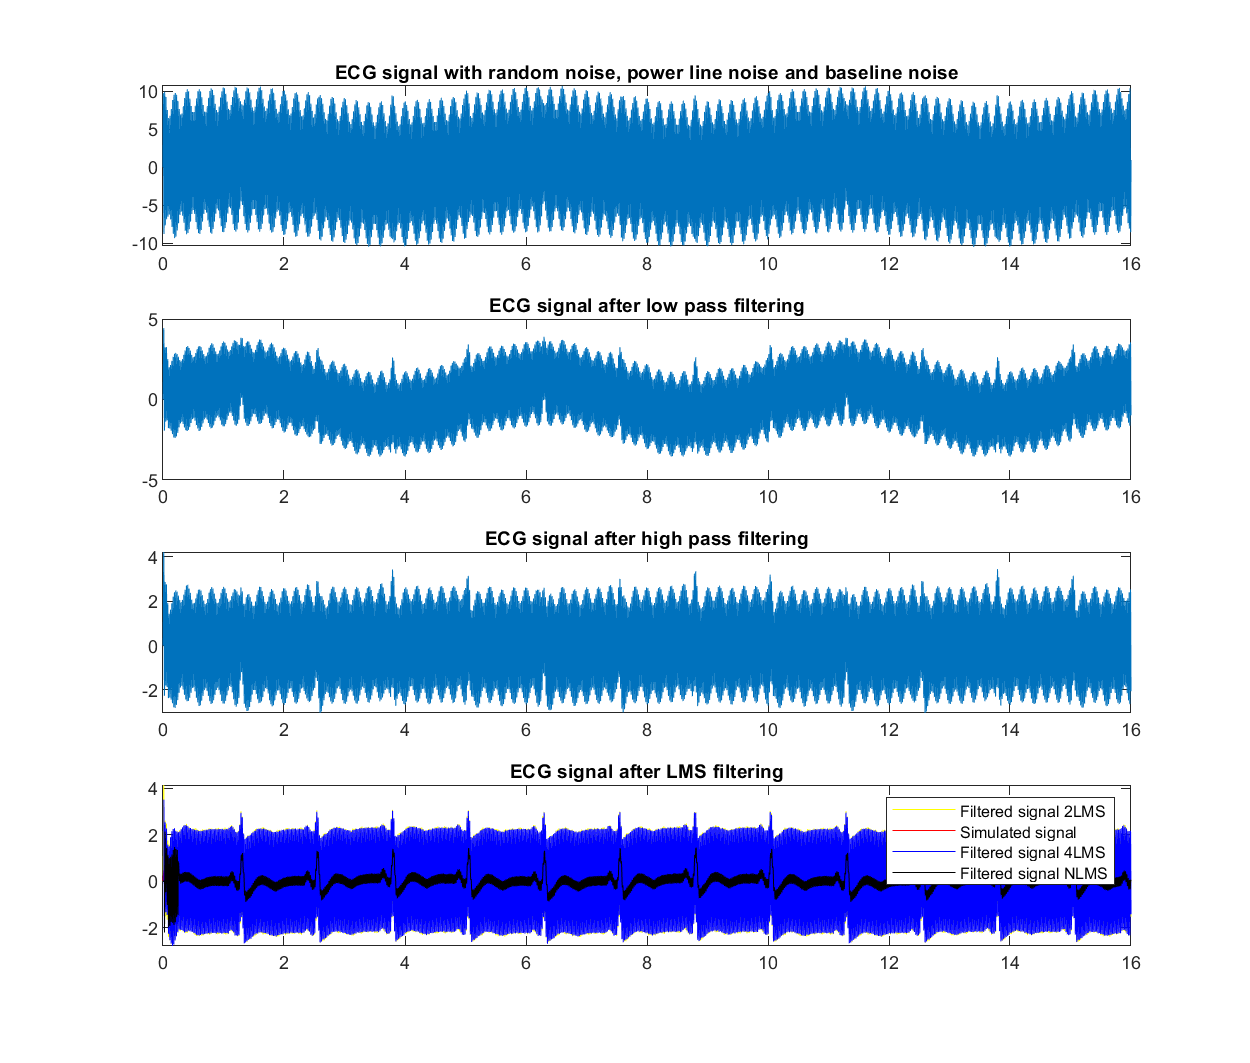
\includegraphics [width=4in]{D:\Facultate\VUB_sem1\Video,Image,Coding Systems\mini-project\Matlab\ECG_N_tap_filter.png}

\end{par} \vspace{1em}



\end{document}

